\documentclass[a4paper]{article}
\usepackage[letterpaper, margin=1in]{geometry} % page format
\usepackage{listings} % this package is for including code
\usepackage{graphicx} % this package is for including figures
\usepackage{amsmath}  % this package is for math and matrices
\usepackage{amsfonts} % this package is for math fonts
\usepackage{tikz} % for drawings
\usepackage{hyperref} % for urls
\usepackage{pdfpages}

\title{Midterm Exam}
\author{Max Schemitsch}
\date{3/13/2019}

\begin{document}
\lstset{language=Python}

\maketitle

\section{Problem 1}
\subsection{Pocket Algorithm, w = 0}
Although I couldn't quite get it working, the code from $Midterm\_Problem1a.py$ is similar to what would be required for classification. This uses the PLA algorithm to separate $y=4$ and $y \neq 4$. The resulting classification would look something like this:

\begin{figure}[h]
  \begin{center}
    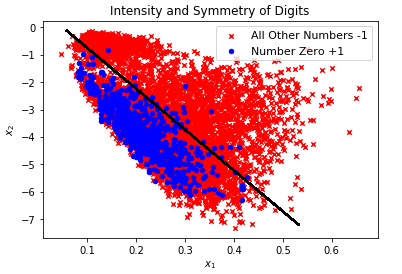
\includegraphics[width=80mm,scale=0.8]{typeA.png}
  \end{center}
\end{figure}

\subsection{Linear Regression}
Similar to Part A, I couldn't get the code working. $Midterm\_Problem1b.py$ replicates a program similar to what would classify this dataset. The result would look something like this:

\begin{figure}[h]
  \begin{center}
    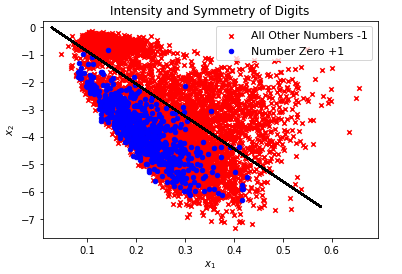
\includegraphics[width=80mm,scale=0.8]{typeB.png}
  \end{center}
\end{figure}

\subsection{Pocket Algorithm, Start with Linear Solution}

Again, I couldn't figure out the code on this one, but I have something that is close to what we would want. $Midterm\_Problem1c.py$ is similar to what would be needed for classification. Our resulting plot would look something like this:

\begin{figure}[h]
  \begin{center}
    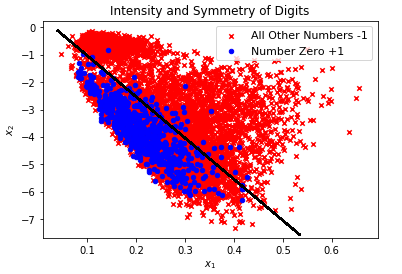
\includegraphics[width=80mm,scale=0.8]{typeC.png}
  \end{center}
\end{figure}

\subsection{Comments}

Even though I couldn't actually run the code, I think the technical best algorithm would be the Pocket Algorithm starting with Linear Regression. This is because it is two programs in one, and may provide a middle-ground solution. Alternatively, the fastest algorithm, as we've discussed in class, is the Linear Regression algorithm. The amount of code and processing time is significantly reduced.

\section{Problem 2}
We can use the code below (from HW2) to solve Problem 2.12 in an iterative manner. \\
I've also added a list, $storedN$, that stores values of $N$ as it iterates. \\
\begin{lstlisting}[frame=single]
import numpy as np
storedN = []
def get_N(dvc=10, delta=0.05, epsilon=0.05, initial_N=1000, tolerance = 1):
    
    new_N = 8 / epsilon**2 * np.log((4 * ((2 * initial_N)**dvc + 1)) / delta)
    storedN.append(new_N)
    
    if abs(new_N - initial_N) < tolerance: # Did it converge?
        return new_N
          
    else: # If so return N
        return get_N(dvc, delta, epsilon, new_N, tolerance) # Iterate

print("Our sample size must be at least " + format(int(get_N())) + ".")
print("Sample Size Estimates: " + str([int(x) for x in storedN]) + ".")
\end{lstlisting}

\begin{lstlisting}
Our sample size must be at least 452956.
Sample Size Estimates: [257251, 434853, 451651, 452864, 452950, 452956, 452956].
\end{lstlisting}

\section{Problem 3 (Extra Credit)}
I like the idea that Marist contains both letters $a$ and $i$, and in order. \\
I'm awful at drawing (especially on a computer), but maybe something like this:
\begin{figure}[h]
  \begin{center}
    
\includegraphics[width=140mm,scale=1]{extracredit.png}
  \end{center}
\end{figure}

\end{document}